\documentclass[12pt]{article}
\usepackage[a4paper, margin=.30in]{geometry}
\usepackage{graphicx ,
            wrapfig,
            xcolor, 
            enumerate,
            amsmath,fontenc,
            tcolorbox,mathrsfs
            }
\usepackage{mathptmx}
\usepackage[siunitx, RPvoltages]{circuitikz}
\newcommand\headerMe[2]{\noindent{}#1\hfill#2}
\renewcommand{\thesection}{\Roman{section}}

\author{Zakaria HAOUZAN}
\date{\today}

\begin{document}
% headers --------------
\headerMe{Matière : Physique-Chimie}{Professeur : Zakaria HAOUZAN}\\
\headerMe{Unité : Electricité}{Établissement : Lycée SKHOR qualifiant}\\
\headerMe{Niveau : 1BAC-SM/X}{Heure : 17H/12H}\\

% ------Content ________

%\begin{wrapfigure}[10]{r}{0.5\textwidth}
    %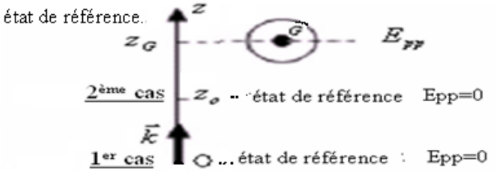
\includegraphics[width=0.5\textwidth]{./img/img00.png}
%\end{wrapfigure}


%\begin{tcolorbox}[colback=black!15!white,
                  %colframe=black!10!black,
                  %title=Remarque :
                 %]
\begin{center}

    \Large{Leçon $N^{\circ} 8 $: \color{red}Forces électromagnétiques }
\end{center}

%\begin{wrapfigure}[5]{r}{0.3\textwidth}
  %\vspace{-3cm}
    %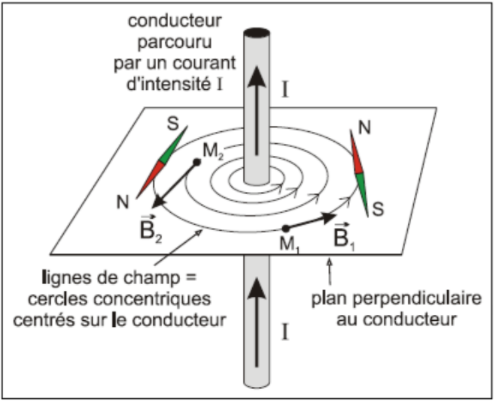
\includegraphics[width=0.3\textwidth]{./img/Un fil de longueur.png}
%\end{wrapfigure}
  \section{ Mise en évidence de la force de Laplace :}
On réalise le montage expérimental suivant en utilisant une tige de cuivre (car le cuivre n'est pas attiré par l'aimant).
La tige est capable de tourner librement autour du point O, son extrémité libre trompe dans le mercure.
  \begin{center}
    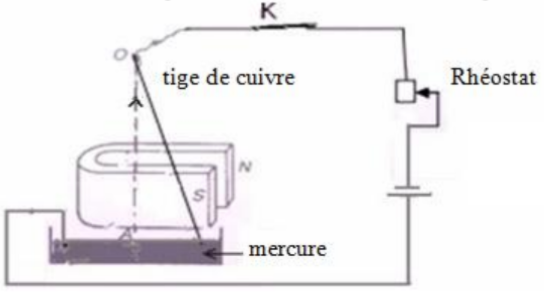
\includegraphics[width=0.3\textwidth]{./img/foce_B.png}
  \end{center}
La tige est placée dans un champ magnétique créé par un aimant en U.
Lorsque l'interrupteur K est ouvert , la tige demeure dans sa position d'équilibre verticale. Lorsqu'on ferme
l'interrupteur K , on constate la que la tige s'incline par rapport à sa position d'équilibre verticale.
En inversant le sens du courant qui traverse la tige , elle s'incline dans le sens contraire.

  \subsection{Interprétation: }
  la tige métallique placée dans un champ $\vec{B}$ et traversée par un courant électrique I est soumise à une force magnétique qu'on appelle force de laplace.
  \subsection{Conclusion:}
  L'orsqu'une partie d'un conducteur métallique de longeur l se trouve dans un champ magnétique $\vec{B}$ et parcourue par un courant électrique d'intensité I, elle est soumise à une force magnétique $\vec{F}$ appelée force de laplace.

  L'expression de la force de laplace est donnée par la relation suivant : $$\vec{F} = I.\vec{l}\wedge \vec{B}$$  
  Le Symbole $\wedge $ représente le produit vectoriel.

  \subsection{Caractéristiques de la force de Laplace:}


-Point d'application: milieu de la portion du conducteur qui se trouve dans le champ magnétique.

-Direction : perpendiculaire au plan déterminé par le conducteur et le vecteur champ magnétique.

  -Sens: il est donné par la règle de la main droite suivante:
En plaçant la main droite de façon que les doigts soient dirigés dans le sens du courant électrique et la paume de main -
dirigée dans le sens du vecteur champ magnétique, le pouce tendu indique le sens la force magnétique.
  \begin{center}

    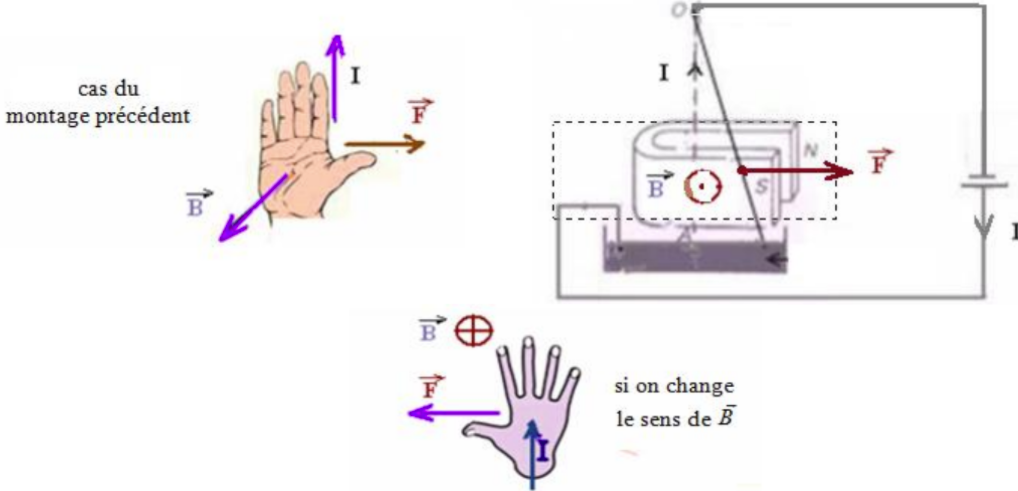
\includegraphics[width=0.7\textwidth]{./img/la force de Laplace_magn.png}
  \end{center}

  -Intensité : l'intensité de la force de laplace $F=B.I.l.sin\alpha$ avec $\alpha = (\vec{B}, \vec{l})$ . $\vec{l}$ étant orienté dans le sens du courant électrique.

  si $\alpha = (\vec{B}, \vec{l}) = \frac{\pi}{2}$ donc $sin\alpha =  1$ par conséquence l'intensité de la force de laplace $F = B.I.l$

  Exemples : Compléter les figures suivantes:
   \begin{center}
    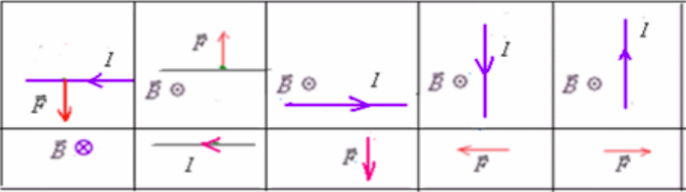
\includegraphics[width=0.6\textwidth]{./img/Exemple_appl.png}
  \end{center}

  \section{Application de la loi de Laplace }
  \subsection{Le haut parleur électrodynamique }
 
Le haut parleur électrodynamique est constitué principalement (figure 5)

• d’un aimant circulaire ;

• d’une bobine circulaire mobile placée autour d’un des pôles de l’aimant ;

• d’une membrane reliée à la bobine ;

• d’un " saladier " ou support qui contient l’aimant, la bobine et la membrane.

Les fils de la bobine sont connectés à la sortie du haut-parleur.
   \begin{center}
    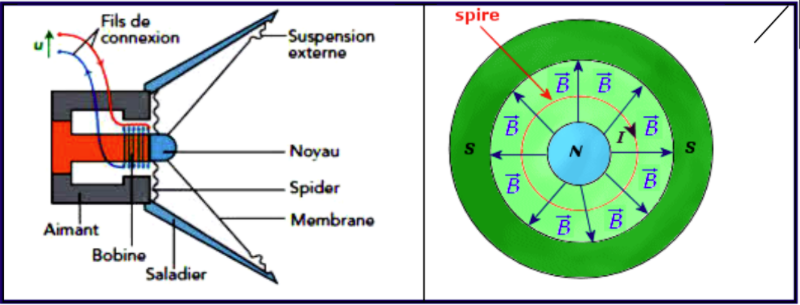
\includegraphics[width=0.4\textwidth]{./img/haut parleur.png}
  \end{center}
Le champ magnétique créé par l’aimant est perpendiculaire en tout point au courant qui circule dans chacune
des spires.
\subsubsection{Principe de fonctionnement du haut-parleur }

Lorsqu'un courant électrique d'intensité I passe dans la bobine, chacune de ses spires est soumise à la force de Laplace qui la met en mouvement ce qui provoque le mouvement de membrane qui agit sur la couche d'air qui
l'entoure et elle produit un son qui a la même fréquence que celle du courant électrique.

   \begin{center}
    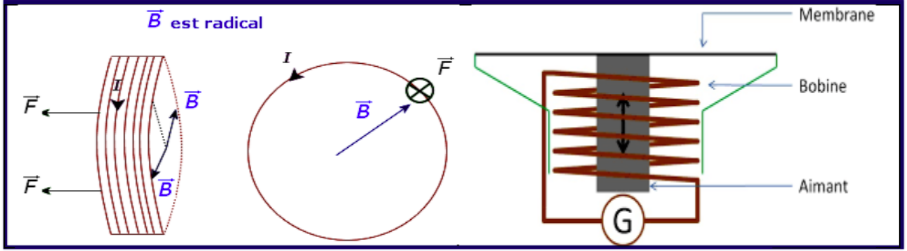
\includegraphics[width=0.7\textwidth]{./img/fonction_haut_par.png}
  \end{center}

L’énergie électrique est transformée en énergie mécanique puis en énergie sonore.

\subsection{Le moteur électrique à courant continue:}
Il est constitué de deux parties essentielles:
\\Le stator: c’est un aimant fixe qui crée un champ magnétique autour de lui.
\\Le rotor : c'est la partie mobile, elle a une forme cylindrique, c'est une association de spires mobiles autour d'un axe.

Dans Le moteur électrique à courant continue ce sont les forces de Laplace qui entraine la rotation.

Le moteur le plus simple est constitué d’un cadre rectangulaire pouvant tourner autour d’un axe . (voir schéma ci-dessous)

   \begin{center}
    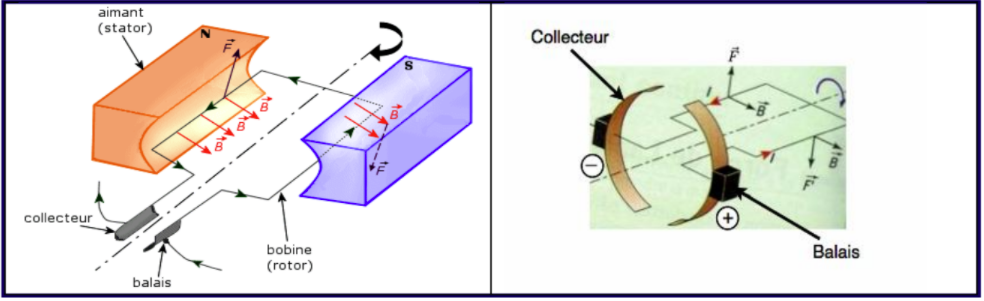
\includegraphics[width=0.7\textwidth]{./img/mcc_app.png}
  \end{center}

\section{Le couplage électromagnétique : (SM)}
\subsection{Transformation de l'énergie électrique en énergie mécanique:}
\subsubsection{Rails de Laplace:}
Une tige de longeur l placée dans un champ magnétique $\vec{B}$, et parcourue par un courant électrique d'intensité I se déplace sur une rails parallèles et horizontale sous l'action de la fore de laplace perpendiculaire à la tige d'intensité F= B.I.l 

   \begin{center}
    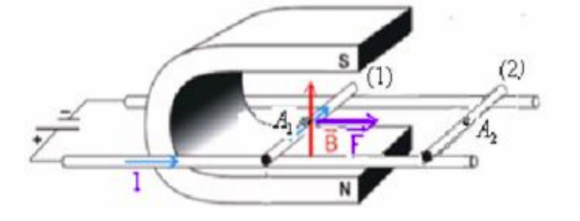
\includegraphics[width=0.5\textwidth]{./img/rail_laplce.png}
  \end{center}
Le travail de cette force durant le déplacement de la position (1) à la position (2) est:
$$W(\vec{F}) = \vec{F}.\vec{A_1A_2} = F.A_1A_2.cos(0) = B.I.l.d$$ 
avec $A_1A_2 = d$ et $W(\vec{F}) > 0$ travail moteur 
Dans cette expérience l'énergie électrique est transformée en énergie mécanique.

Conclusion : Une partie de l’énergie électrique fournie par le générateur est convertie en énergie mécanique .

Le moteur reçoit pendant une durée $\Delta{t}$ une énergie électrique $W_e = U.I.\Delta{t}$, il se transforme une partie de cette énergie en énergie mécanique $W_m$ et d'autre partie est dissipée par frottement sous forme d'énergie thermique par effet de Joule .

Le rendement du moteur est : $\rho = \frac{W_m}{W_e}$. C’est le principe des moteurs à courant continu.

\subsection{Transformation de l'énergie mécanique en énergie électrique:}
En déplaçant un aimant près d'une bobine lié à un ampèremètre ou en déplaçant la tige sur deux rails liés à un
ampèremètre et placées dans un champ magnétique on constate l'apparition d'un courant électrique dans le circuit.
   \begin{center}
    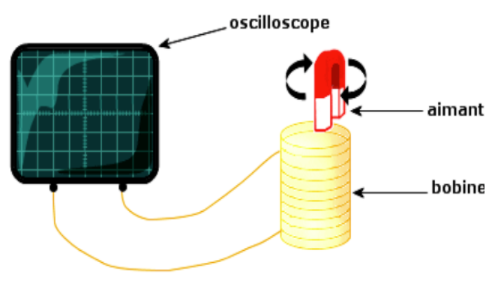
\includegraphics[width=0.5\textwidth]{./img/app_elec.png}
  \end{center}
Dans cette expérience l'énergie mécanique est transformée en énergie électrique.

Conclusion:

Les moteurs électriques et les haut- parleurs transforment l'énergie électrique qu'ils reçoivent en énergie mécanique
grâce à la force de Laplace.

Ce transfert de l'énergie électrique en énergie mécanique (ou l'inverse dans d'autre appareil) est connu sous le nom : Couplage électrodynamique.

(Signalons que cette transformation est presque totale car l'énergie perdue par frottement par effet Joule est très faible
devant l'énergie reçue).



\end{document}

